
\let\negmedspace\undefined
\let\negthickspace\undefined
\documentclass[journal]{IEEEtran}
\usepackage[a5paper, margin=10mm, onecolumn]{geometry}
%\usepackage{lmodern} % Ensure lmodern is loaded for pdflatex
\usepackage{tfrupee} % Include tfrupee package
\setlength{\headheight}{1cm} % Set the height of the header box
\setlength{\headsep}{0mm}     % Set the distance between the header box and the top of the text
\usepackage{gvv-book}
\usepackage{gvv}
\usepackage{cite}
\usepackage{amsmath,amssymb,amsfonts,amsthm}
\usepackage{algorithmic}
\usepackage{graphicx}
\usepackage{textcomp}
\usepackage{xcolor}
\usepackage{txfonts}
\usepackage{listings}
\usepackage{enumitem}
\usepackage{mathtools}
\usepackage{gensymb}
\usepackage{comment}
\usepackage[breaklinks=true]{hyperref}
\usepackage{tkz-euclide} 
\usepackage{listings}
% \usepackage{gvv}                                        
\def\inputGnumericTable{}                                 
\usepackage[latin1]{inputenc}                                
\usepackage{color}                                            
\usepackage{array}                                            
\usepackage{longtable}                                       
\usepackage{calc}                                             
\usepackage{multirow}                                         
\usepackage{hhline}                                           
\usepackage{ifthen}                                           
\usepackage{lscape}
\renewcommand{\thefigure}{\theenumi}
\renewcommand{\thetable}{\theenumi}
\setlength{\intextsep}{10pt} % Space between text and floats
\numberwithin{equation}{enumi}
\numberwithin{figure}{enumi}
\renewcommand{\thetable}{\theenumi}
\begin{document}
\bibliographystyle{IEEEtran}
\title{11.16.3.7}
\author{EE24BTECH11041 - Mohit}
% \maketitle
% \newpage
% \bigskip
{\let\newpage\relax\maketitle}
\textbf{Question:-} A fair coin is tossed four times, and a person wins Rs.1 for each head and loses Rs.1.50 for each tail. From the sample space, calculate how many different amounts of money you can have after four tosses and the probability of having each of these amounts.

\textbf{Solution}

Let:
\begin{align}
H = +1 \quad \text{(gain Rs.1 for Head)}, \quad T = -1.50 \quad \text{(lose Rs.1.50 for Tail)}.
\end{align}

For $ x $, the number of heads in 4 tosses, the total net money can be calculated using the formula:
\begin{align}
\text{Net Money} = x(1) + (4-x)(-1.5)\\
\text{Net Money} = x - 1.5(4-x)\\
\text{Net Money} = 2.5x - 6,
\end{align}

where $ x = 0, 1, 2, 3, 4 $.

\textbf{Possible Outcomes and Net Money}

\begin{itemize}
    \item $ x = 0 $: All tails ($ TTTT $):
    \begin{align}
    \text{Net Money} = 2.5(0) - 6 = -6
    \end{align}
    \item $ x = 1 $: One head, three tails ($ HTTT, THTT, TTHT, TTTH $, etc.):
    \begin{align}
    \text{Net Money} = 2.5(1) - 6 = -3.5
    \end{align}
    \item $ x = 2 $: Two heads, two tails ($ HHTT, HTHT, HTTH, \dots $):
    \begin{align}
    \text{Net Money} = 2.5(2) - 6 = -1
    \end{align}
    \item $ x = 3 $: Three heads, one tail ($ HHHT, HHTH, HTHH, THHH $):
    \begin{align}
    \text{Net Money} = 2.5(3) - 6 = 1.5
    \end{align}
    \item $ x = 4 $: All heads ($ HHHH $):
    \begin{align}
    \text{Net Money} = 2.5(4) - 6 = 4
    \end{align}
\end{itemize}

\textbf{Number of Outcomes for Each Case}

The number of outcomes for each $ x $ is given by the binomial coefficient $ \binom{4}{x} $:

\begin{align}
    &x = 0: \binom{4}{0} = 1, \\
    &x = 1: \binom{4}{1} = 4, \\
    &x = 2: \binom{4}{2} = 6, \\
    &x = 3: \binom{4}{3} = 4, \\
    &x = 4: \binom{4}{4} = 1
\end{align}

\textbf{Probabilities of Each Case}

Since the coin is fair, the probability of each outcome is $ \frac{1}{16} $. The probabilities for each $ x $ are:

\begin{align}
    &x = 0: \text{Probability} = \frac{\binom{4}{0}}{16} = \frac{1}{16}, \\
    &x = 1: \text{Probability} = \frac{\binom{4}{1}}{16} = \frac{4}{16} = \frac{1}{4}, \\
    &x = 2: \text{Probability} = \frac{\binom{4}{2}}{16} = \frac{6}{16} = \frac{3}{8}, \\
    &x = 3: \text{Probability} = \frac{\binom{4}{3}}{16} = \frac{4}{16} = \frac{1}{4}, \\
    &x = 4: \text{Probability} = \frac{\binom{4}{4}}{16} = \frac{1}{16}.
\end{align}


\textbf{CODING LOGIC:-}



A fair coin is tossed 4 times, and the outcomes are:
\begin{itemize}
    \item Heads $(H)$: Gain Rs.1.
    \item Tails $(T)$: Lose Rs.1.50.
\end{itemize}

Define $X_i$ as the random variable for the net money from the $i$-th toss:
\begin{align}
X_i =
\begin{cases}
1, & \text{if Head (H)} \quad \big(P(X_i = 1) = 0.5\big) \\
-1.5, & \text{if Tail (T)} \quad \big(P(X_i = -1.5) = 0.5\big)
\end{cases}
\end{align}

The total net money after 4 tosses is:
\begin{align}
S = \sum_{i=1}^4 X_i
\end{align}

\textbf{Z-Transform of a Single Toss}

The Z-transform of a random variable is defined as:
\begin{align}
G_X(z) = \mathbb{E}[z^X]
\end{align}
where $\mathbb{E}[\cdot]$ is the expectation operator. For $X_i$, the Z-transform is:
\begin{align}
G_{X_i}(z) = P(X_i = 1)z^1 + P(X_i = -1.5)z^{-1.5}\\
G_{X_i}(z) = 0.5z + 0.5z^{-1.5}
\end{align}

\textbf{Z-Transform of Total Net Money}

Since the tosses are independent, the Z-transform of the total net money $S$ is the product of the Z-transforms of individual tosses:
\begin{align}
G_S(z) = \big(G_{X_i}(z)\big)^4 \\
G_S(z) = \big(0.5z + 0.5z^{-1.5}\big)^4
\end{align}

\textbf{Expansion of the Z-Transform}

Using the binomial theorem, expand $G_S(z)$:
\begin{align}
G_S(z) = \sum_{k=0}^4 \binom{4}{k} \big(0.5z\big)^k \big(0.5z^{-1.5}\big)^{4-k} \\
G_S(z) = \sum_{k=0}^4 \binom{4}{k} (0.5)^4 z^{k - 1.5(4-k)} \\
G_S(z) = \sum_{k=0}^4 \binom{4}{k} (0.5)^4 z^{2.5k - 6}
\end{align}

The coefficients of $z^m$ in this expansion represent the probabilities $P(S = m)$, i.e., the PMF.

\textbf{Net Money Values and PMF}

The possible net money values are:
\begin{align}
S \in \{-6, -3.5, -1, 1.5, 4\}
\end{align}

Substituting these values into the expansion of $G_S(z)$, the probabilities are:
\begin{align}
P(S = -6) = \frac{1}{16}, \quad P(S = -3.5) = \frac{4}{16}, \quad P(S = -1) = \frac{6}{16}, \quad P(S = 1.5) = \frac{4}{16}, \quad P(S = 4) = \frac{1}{16}
\end{align}

Thus, the PMF is:
\begin{align}
P(S = x) =
\begin{cases}
\frac{1}{16}, & x = -6 \\
\frac{4}{16}, & x = -3.5 \\
\frac{6}{16}, & x = -1 \\
\frac{4}{16}, & x = 1.5 \\
\frac{1}{16}, & x = 4 \\
0, & \text{otherwise}
\end{cases}
\end{align}



\textbf{CDF of $S$}

The Cumulative Distribution Function (CDF) is defined as:
\begin{align}
F(x) = P(S \leq x) = \sum_{k \leq x} P(S = k)
\end{align}

The possible values of $S$ and the corresponding CDF values are:
\begin{itemize}
    \item For $x < -6$:
    \begin{align}
    F(x) = 0
    \end{align}
    \item For \(-6 \leq x < -3.5\):
    \begin{align}
    F(x) = P(S = -6) = \frac{1}{16}
    \end{align}
    \item For \(-3.5 \leq x < -1\):
    \begin{align}
    F(x) = P(S = -6) + P(S = -3.5) = \frac{1}{16} + \frac{4}{16} = \frac{5}{16}
    \end{align}
    \item For \(-1 \leq x < 1.5\):
    \begin{align}
    F(x) = P(S = -6) + P(S = -3.5) + P(S = -1) = \frac{1}{16} + \frac{4}{16} + \frac{6}{16} = \frac{11}{16}
    \end{align}
    \item For \(1.5 \leq x < 4\):
    \begin{align}
    F(x) = P(S = -6) + P(S = -3.5) + P(S = -1) + P(S = 1.5) = \frac{1}{16} + \frac{4}{16} + \frac{6}{16} + \frac{4}{16} = \frac{15}{16}
    \end{align}
    \item For \(x \geq 4\):
    \begin{align}
    F(x) = 1
    \end{align}
\end{itemize}

Thus, the CDF is:
\begin{align}
F(x) =
\begin{cases}
0, & x < -6 \\
\frac{1}{16}, & -6 \leq x < -3.5 \\
\frac{5}{16}, & -3.5 \leq x < -1 \\
\frac{11}{16}, & -1 \leq x < 1.5 \\
\frac{15}{16}, & 1.5 \leq x < 4 \\
1, & x \geq 4
\end{cases}
\end{align}

\begin{figure}[h!]
   \centering
   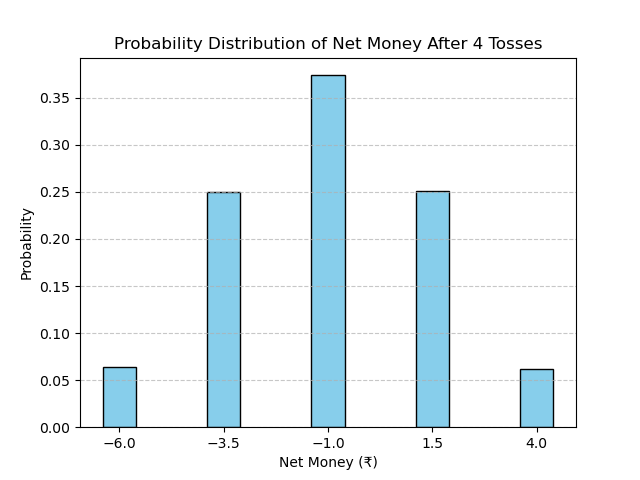
\includegraphics[width=0.7\linewidth]{figs/Figure_1.png}
\end{figure}

\end{document}
